\documentclass[a4paper,11pt]{article}
\usepackage[margin=2.5cm]{geometry}
\usepackage{amsmath,amssymb,graphicx,booktabs,hyperref}
\hypersetup{colorlinks=true,linkcolor=black,citecolor=black,urlcolor=black}
\title{Attention Mechanisms:\\From Sequences to Document Understanding}
\author{Mopai Research Studio}
\date{A complete, editable sample project}
\begin{document}
\maketitle
\begin{abstract}
Attention provides a direct way to represent dependencies between elements of a sequence. This note introduces scaled dot-product attention and illustrates its computation with an embedded figure and a verification table. The project demonstrates how editable equations, images, cross-references and bibliography entries can coexist in a complete, reproducible \LaTeX{} document.
\end{abstract}
\noindent\textbf{Keywords:} attention; sequence modeling; document understanding; typesetting
\section{Introduction}
A research document communicates through more than paragraphs. Equations express precise relationships; figures reveal structure; tables support comparison; citations connect claims to their sources. A reliable typesetting workflow must preserve these elements while giving them a clear visual hierarchy.
The Transformer uses attention to model dependencies within a sequence\cite{vaswani2017}. Here, its core equation serves as a compact example of mathematical content that should remain editable throughout document conversion.
\section{Scaled Dot-Product Attention}
Let $Q$, $K$ and $V$ denote the query, key and value matrices, and let $d_k$ be the dimensionality of the keys. Scaled dot-product attention is defined as
\begin{equation}
\operatorname{Attention}(Q,K,V)=\operatorname{softmax}\!\left(\frac{QK^{\mathsf T}}{\sqrt{d_k}}\right)V.
\label{eq:attention}
\end{equation}
Equation~\eqref{eq:attention} first measures the similarity between queries and keys. The scores are scaled, normalized, and then used to compute a weighted combination of values. The matrix operations can be evaluated in parallel.
\begin{figure}[htbp]
\centering
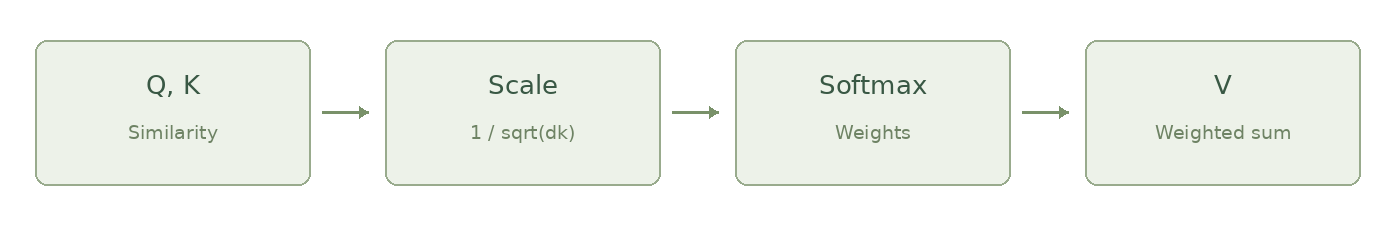
\includegraphics[width=0.92\linewidth]{figures/attention.png}
\caption{The computational stages of scaled dot-product attention.}
\label{fig:attention}
\end{figure}
Figure~\ref{fig:attention} keeps the diagram as a project-local image while maintaining the caption and label as editable source text.
\section{Checking Structure and Content}
Compilation is a necessary technical check, but a valid PDF can still contain transcription mistakes. Table~\ref{tab:checks} separates basic automated checks from content review.
\begin{table}[htbp]
\centering
\caption{Different checks for different parts of a document.}
\label{tab:checks}
\begin{tabular}{lll}
\toprule
Element & Automated check & Content review \\
\midrule
Equation & Syntax and compilation & Symbols and subscripts \\
Figure & File path and embedding & Crop and caption alignment \\
Citation & Resolved commands & Source correspondence \\
\bottomrule
\end{tabular}
\end{table}
A reproducible project should retain its source, image assets, bibliography and actual compilation logs. Any unresolved uncertainty should remain visible in the delivery report.
\section{Conclusion}
Good typesetting gives careful ideas a clear form. A complete engineering workflow combines compilation, structural checks and explicit content review, and never treats a successful build as proof of semantic fidelity.
\begin{thebibliography}{9}
\bibitem{vaswani2017}
A. Vaswani, N. Shazeer, N. Parmar, et al.
\textit{Attention Is All You Need}.
Advances in Neural Information Processing Systems, 2017.
\end{thebibliography}
\end{document}
